\documentclass[10pt,twocolumn,a4paper]{article}
 
\usepackage[utf8]{inputenc}
\usepackage[T1]{fontenc}
\usepackage[top=0.8in,bottom=0.9in,left=0.65in,right=0.65in,columnsep=0.25in]{geometry}
\usepackage{mathptmx}          % Times text and math (IEEE look)
\usepackage{microtype}
\usepackage{amsmath,amssymb}
\usepackage{cite}
\usepackage{booktabs}
\usepackage{multirow}
\usepackage{graphicx}
\usepackage{listings}
\usepackage{xcolor}
\usepackage{tikz}
\usepackage{pgfplots}
\pgfplotsset{compat=1.16}
\usetikzlibrary{arrows.meta,positioning,shapes.geometric,fit,calc}
\usepackage{enumitem}
\usepackage{titlesec}
\usepackage[font=footnotesize,labelsep=period,justification=justified,singlelinecheck=true]{caption}
\captionsetup[table]{labelsep=newline,labelfont=sc,textfont=sc,justification=centering,skip=4pt}
\captionsetup[figure]{name={Fig.}}
\usepackage[hidelinks]{hyperref}
 
\setlist{itemsep=1pt,topsep=3pt,parsep=0pt,leftmargin=1.4em}
\setlength{\parindent}{1em}
\setlength{\parskip}{0pt}
\emergencystretch=2em
\setlength{\abovedisplayskip}{4pt}
\setlength{\belowdisplayskip}{4pt}
\setlength{\abovedisplayshortskip}{2pt}
\setlength{\belowdisplayshortskip}{2pt}
 
% ---- IEEE-style section headings
\renewcommand{\thesection}{\Roman{section}}
\renewcommand{\thesubsection}{\Alph{subsection}}
\renewcommand{\refname}{References}
\titleformat{\section}{\centering\footnotesize\scshape}{\thesection.}{0.6em}{\MakeUppercase}
\titlespacing*{\section}{0pt}{10pt}{4pt}
\titleformat{\subsection}{\normalsize\itshape}{\thesubsection.}{0.5em}{}
\titlespacing*{\subsection}{0pt}{6pt}{2pt}
\titleformat{\paragraph}[runin]{\itshape}{}{0pt}{}[.\ ]
\titlespacing*{\paragraph}{\parindent}{4pt}{0.5em}
 
\lstdefinelanguage{SPARQL}{
  morekeywords={SELECT,WHERE,PREFIX,ASK,FILTER,ORDER,BY,SERVICE,CONTAINS,LCASE,DISTINCT},
  sensitive=false,
  morecomment=[l]{\#}
}
\lstset{
  language=SPARQL,
  basicstyle=\ttfamily\scriptsize,
  keywordstyle=\bfseries,
  frame=single,
  breaklines=true,
  columns=fullflexible,
  xleftmargin=0.3em,
  xrightmargin=0.3em,
  aboveskip=4pt,
  belowskip=4pt
}
 
% Notation shortcuts
\renewcommand{\bowtie}{\mathrel{\triangleright\!\triangleleft}}
\newcommand{\NDTL}{\textsc{NDTL}}
\newcommand{\SKG}{S_{\mathrm{KG}}}
 
\makeatletter
\begin{document}
 
\twocolumn[{%
\begin{@twocolumnfalse}
\begin{center}
{\fontsize{19}{23}\selectfont \textbf{Logic-Based Analysis of Fake News Diffusion on Social Media:}}\\[4pt]
{\fontsize{13}{17}\selectfont Reproduction, Linear-Time Verification, and Knowledge-Graph Grounding}\\[10pt]
{\large Keerthana V K\textsuperscript{1}\hspace{2em} Anusree S\textsuperscript{1}\hspace{2em} Sishu Shankar Muni\textsuperscript{1}}\\[4pt]
{\small\itshape \textsuperscript{1}Kerala University of Digital Sciences, Innovations and Technology\\ (Digital University Kerala), Kerala, India}
\end{center}
\vspace{4pt}
\begin{center}
\begin{minipage}{0.92\textwidth}
\footnotesize
\noindent\textit{Abstract}---Formal temporal-logic approaches to fake-news detection, such as News-Diffusion Temporal Logic (\NDTL)~\cite{fionda2025}, provide mathematically transparent explanations of cascade propagation but remain content-blind, which leaves them vulnerable to false alarms on viral breaking news. This paper presents an integrated framework bridging Social Network Analysis and the Semantic Web. We first perform an independent re-implementation of \NDTL, resolving a redundant path-traversal bottleneck in the reference model checker via a linear-time Breadth-First Search (BFS) evaluator that reduces verification runtime to 9.2\,ms per cascade on commodity hardware. Second, to address the content-agnostic limitation of \NDTL, we introduce a Semantic Web Knowledge Graph (KG) fact-checking engine that extracts factual assertions and queries public Wikidata and DBpedia endpoints via SPARQL, achieving an isolated fake-class precision of 96.5\% at 54.2\% recall on Twitter16. Third, we formalize diffusion cascades as W3C Linked Data using the PROV-O ontology and the SIOC vocabulary, enabling direct SPARQL querying over propagation trees. Finally, we fuse temporal diffusion dynamics with semantic signals in a symbolic-statistical hybrid classifier. Under stratified 10-fold cross-validation, the hybrid improves accuracy over our reproduced \NDTL\ baseline by 26.8 percentage points (53.7\% to 80.5\%, relative gain +49.8\%) on Twitter16 and by 18.7 percentage points (53.2\% to 71.9\%, relative gain +35.2\%) on Twitter15, while Twitter15 Fake recall decreases from 0.796 to 0.610. The proposed system provides human-interpretable structural and semantic evidence; it improves significantly over the reproduced logic baseline while remaining lightweight compared to deep sequence models.
 
\vspace{4pt}
\noindent\textit{Index Terms}---fake news detection, information diffusion, temporal logic, knowledge graph, Semantic Web, SPARQL, social network analysis.
\end{minipage}
\end{center}
\vspace{10pt}
\end{@twocolumnfalse}
}]
\makeatother
 
%---------------------------------------------------------------------
\section{Introduction}
Social media networks have become the primary channel for information dissemination, yet they simultaneously facilitate the rapid propagation of fabricated, misleading, and unverified claims. Empirical studies by Vosoughi et al.~\cite{vosoughi2018} demonstrate that false news diffuses significantly deeper, faster, and more broadly than truthful information. Pioneering analyses by Castillo et al.~\cite{castillo2011} and Kwon et al.~\cite{kwon2013rumor} further established that structural and temporal characteristics of information cascades provide early discriminative signals of rumor spread, motivating comprehensive data-mining frameworks~\cite{shu2017mining}.

Conventional detection paradigms predominantly focus on content-based analysis, employing natural language processing (NLP) and large language models (LLMs) to inspect linguistic markers, emotional sentiment, and sensationalism. However, content-based approaches remain vulnerable to adversarial text perturbation, multilingual shifts, and automated generation by generative AI. Consequently, modern research has shifted toward context-based and diffusion-based approaches, which analyze the topological and temporal structures of information propagation cascades. Despite their empirical success, contemporary graph neural networks (GNNs)~\cite{bian2020, dou2021upfd, nguyen2020fang}, recurrent architectures~\cite{ma2016, liu2018ppc, ruchansky2017csi}, and recursive tree models~\cite{ma2018rvnn, lu2020gcan} suffer from the ``black-box'' dilemma: they generate probabilistic veracity predictions without auditable, human-interpretable justifications.

To address this challenge, Fionda~\cite{fionda2025} proposed News-Diffusion Temporal Logic (\NDTL), a formal verification language tailored for social media cascades. \NDTL\ synthesizes human-readable temporal formulas that explicitly capture diffusion velocity, neighborhood structural depth, and spread rate.

Throughout this paper, \emph{re-implementation} refers to reconstructing \NDTL\ from its published formal description using our own codebase evaluated on the same benchmark datasets. In this work, we present:
\begin{enumerate}
  \item An independent re-implementation of the \NDTL\ pipeline, parser, metric computation, and model checking modules, quantifying deviations from published metrics.
  \item Algorithmic optimization of the model checker, resolving redundant subtree re-traversals via an $O(|\varphi| \cdot |N|)$ BFS evaluator ($9.2$\,ms per cascade on commodity hardware).
  \item Evaluation on synthetic networks and on the empirical Twitter15 and Twitter16 benchmarks~\cite{ma2016, ma2017}, validating published diffusion trends.
  \item A Semantic Web Knowledge Graph fact-checking engine over Wikidata~\cite{vrandecic2014} and DBpedia~\cite{lehmann2015} with PROV-O~\cite{lebo2013} and SIOC cascade modeling, fused into a symbolic-statistical hybrid classifier that increases accuracy to 80.5\% on Twitter16 and 71.9\% on Twitter15.
\end{enumerate}

\section{Related Work}
\paragraph{Information Diffusion Modeling and Point Processes}
Pioneering work by Castillo et al.~\cite{castillo2011} demonstrated that temporal characteristics of retweets are highly informative regarding rumor credibility. Vosoughi et al.~\cite{vosoughi2018} analyzed 126,000 rumor cascades on Twitter and observed that fake cascades exhibit significantly higher topological depth and early velocity. Goel et al.~\cite{goel2015structural} formalized structural virality, showing how cascade geometries differentiate viral broadcast phenomena from multi-generational peer diffusion. To model the bursty temporal arrival of cascading posts, point processes have been widely explored: Zhao et al.~\cite{zhao2015seismic} introduced SEISMIC, a self-exciting Hawkes process predicting cascade sizes; Farajtabar et al.~\cite{farajtabar2017fake} formulated point-process interventions to mitigate rumor spread; Mishra et al.~\cite{mishra2016feature} combined temporal delay markers with statistical predictors; and Wu et al.~\cite{wu2015weibo} investigated structural patterns across microblog diffusion networks.

\paragraph{Propagation Structures and Graph Neural Networks}
Early rumor detection architectures relied on hand-crafted temporal features~\cite{kwon2013rumor} and recurrent sequence modeling; Ma et al.~\cite{ma2016} employed GRUs to process continuous time windows of tweet replies. Subsequent research incorporated explicit propagation trees: Ma et al.~\cite{ma2017} developed Propagation Tree Kernels (PTK) to capture subtree similarities, and later introduced Tree-structured Recursive Neural Networks (TD-RvNN and BU-RvNN)~\cite{ma2018rvnn} to model top-down and bottom-up information flows. Liu and Wu~\cite{liu2018ppc} proposed the Propagation Path Classifier (PPC), combining RNNs and CNNs over paths to identify early disinformation. More recently, Graph Convolutional Networks (GCNs) have become predominant: Bian et al.~\cite{bian2020} introduced Bi-GCN to capture both diffusion spreading and response aggregation; Lu and Li~\cite{lu2020gcan} developed GCAN using graph-aware co-attention networks to highlight suspect propagation pathways; Dou et al.~\cite{dou2021upfd} formulated UPFD to combine user preferences with tree-structured GNNs; and Nguyen et al.~\cite{nguyen2020fang} presented FANG, learning graph representations over users, entities, and citations. Contextual and multimodal models like CSI~\cite{ruchansky2017csi} and dEFEND~\cite{shu2019defend} further demonstrate the discriminative power of propagation context.

\paragraph{Formal Verification and Temporal Logics on Networks}
Temporal logics, including Linear Temporal Logic (LTL) and Computation Tree Logic (CTL), have long been applied in formal software and system verification. To monitor continuous real-valued signals, Maler and Nickovic developed Metric Temporal Logic (MTL), later generalized into Signal Temporal Logic (STL) for cyber-physical monitoring~\cite{bartocci2018stl}. Spatial and spatio-temporal logics have subsequently been extended to complex networks and biological systems; Nenzi et al.~\cite{nenzi2015sstl} formulated Spatial-Temporal Logic (SSTL) to evaluate properties over spatial graphs. Building upon this formal trajectory, Fionda~\cite{fionda2025} proposed News-Diffusion Temporal Logic (\NDTL), formalizing directed social diffusion cascades via multi-hop neighborhood modalities ($\Gamma^i$) and statistical aggregation operators ($\max$, $\min$, $\mathrm{avg}$). Unlike deep models, \NDTL\ yields human-readable logic specifications, although its native model checking algorithm suffered from recursive subtree re-traversals that we resolve herein.

\paragraph{Knowledge Graphs and Semantic Fact-Checking}
The Semantic Web vision~\cite{berners2001} provides standard ontologies and structured knowledge bases that facilitate automated factual reasoning. Open knowledge graphs such as Wikidata~\cite{vrandecic2014} and DBpedia~\cite{lehmann2015} represent verified world knowledge as entity--relation triples $(h,r,t)$. Ciampaglia et al.~\cite{ciampaglia2015} demonstrated computational fact-checking by computing shortest paths and transitive closures over knowledge networks, while Shiralkar et al.~\cite{shiralkar2017kgminer} developed KGMiner to evaluate maximum-flow paths. Benchmark initiatives like FEVER~\cite{thorne2018fever} formalized claim extraction and verification pipelines. To bridge unstructured text and structured triples, Hu et al.~\cite{hu2021comparenet} introduced CompareNet, comparing claims against directed entity graphs, and Choi et al.~\cite{choi2021cofact} presented CoFact for evidence-based verification. Recent surveys by Pan et al.~\cite{pan2024unifying} emphasize the crucial role of external knowledge graphs in grounding neuro-symbolic reasoning and mitigating hallucination. Our work unites topological diffusion logic with Semantic Web ontologies (PROV-O~\cite{lebo2013} and SIOC) and SPARQL-based fact-checking.

\section{Problem Formulation}
An information cascade is modeled as a directed, attributed tree (Fig.~1)
\begin{equation}
G = (N, E, \lambda, t, \delta, \sigma),
\end{equation}
where $N$ is the set of event nodes (original post, tweets, and retweets), $E \subseteq N \times N$ represents directed transmission edges, and $\lambda : N \to \{\mathrm{Root}, \mathrm{Tweet}, \mathrm{Retweet}\}$ assigns the event type. The temporal dynamics take values in $\mathbb{R}^{\ge 0}$:
\begin{itemize}
  \item $t : N \to \mathbb{R}^{\ge 0}$ assigns the absolute timestamp of the event.
  \item $\delta : N \to \mathbb{R}^{\ge 0}$ assigns the inter-event delay elapsed since activation of parent $u$, where $(u,v)\in E$:
  \begin{equation}
  \delta(v) = t(v) - t(u), \quad \text{with } \delta(v_0) = 0.
  \end{equation}
  \item $\sigma : N \to \mathbb{R}^{\ge 0}$ denotes cumulative elapsed time from root event $v_0$. For a node $v$ reached from $v_0$ through unique tree path $v_0 = w_0, w_1, \dots, w_m = v$,
  \begin{equation}
  \sigma(v) = \sum_{k=1}^{m} \delta(w_k) = t(v) - t(v_0), \quad \text{with } \sigma(v_0) = 0.
  \end{equation}
\end{itemize}
 
\begin{figure}[t]
\centering
\resizebox{\columnwidth}{!}{%
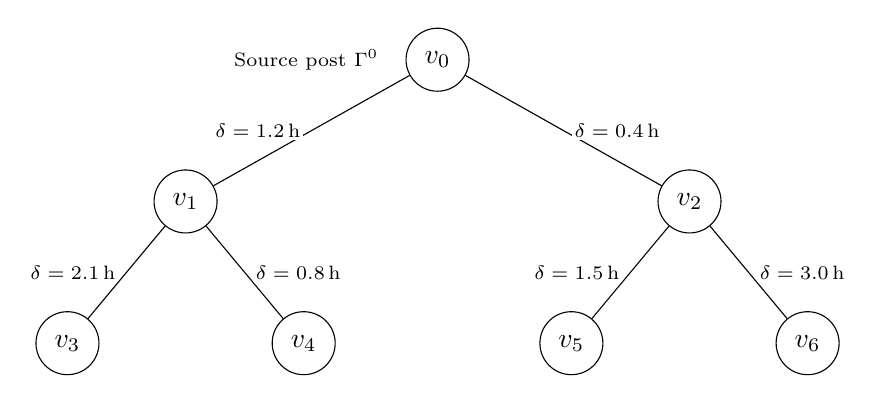
\begin{tikzpicture}[
  every node/.style={circle,draw,minimum size=8mm,inner sep=1pt},
  lbl/.style={draw=none,rectangle,font=\scriptsize,minimum size=0pt,inner sep=1pt,fill=white},
  level 1/.style={sibling distance=64mm,level distance=18mm},
  level 2/.style={sibling distance=30mm,level distance=18mm}]
  \node (v0) {$v_0$}
    child { node (v1) {$v_1$}
      child { node (v3) {$v_3$} edge from parent node[lbl,midway,left=1mm] {$\delta=2.1$\,h} }
      child { node (v4) {$v_4$} edge from parent node[lbl,midway,right=1mm] {$\delta=0.8$\,h} }
      edge from parent node[lbl,midway,left=1mm] {$\delta=1.2$\,h} }
    child { node (v2) {$v_2$}
      child { node (v5) {$v_5$} edge from parent node[lbl,midway,left=1mm] {$\delta=1.5$\,h} }
      child { node (v6) {$v_6$} edge from parent node[lbl,midway,right=1mm] {$\delta=3.0$\,h} }
      edge from parent node[lbl,midway,right=1mm] {$\delta=0.4$\,h} };
  \node[lbl,left=3mm of v0] {Source post $\Gamma^0$};
\end{tikzpicture}}
\caption{Directed diffusion tree $G=(N,E,\lambda,t,\delta,\sigma)$. Edge label on $(u,v)$ denotes delay $\delta(v)$ in hours; $\Gamma^0(v_0)=\{v_0\}$, and $v_1,v_2$ form hop-1 neighborhood $\Gamma^1(v_0)$. E.g., cumulative time $\sigma(v_3) = \delta(v_1) + \delta(v_3) = 1.2 + 2.1 = 3.3$\,h.}
\label{fig:tree}
\end{figure}
 
The $i$-hop neighborhood $\Gamma^i(v)$ of node $v$ is defined as
\begin{equation}
\Gamma^i(v) = \{\, u \in N \mid d(v,u) = i \,\},
\end{equation}
where $d(v,u)$ is the shortest directed tree distance in $G$, with $\Gamma^0(v)=\{v\}$. The complete descendant cascade is denoted $\Gamma^{\infty}(v) = \bigcup_{i=1}^{\infty}\Gamma^i(v)$.
 
%---------------------------------------------------------------------
\section{News-Diffusion Temporal Logic}
\subsection{Syntax and Semantics}
\NDTL\ formulas are inductively defined over atomic predicates according to the following grammar:
\begin{align}
\varphi ::={}& e \mid \rho \bowtie \epsilon \mid (\rho_1 \pm \rho_2)\bowtie\epsilon \mid \neg\varphi \nonumber\\
& \mid \varphi_1\wedge\varphi_2 \mid \varphi_1\vee\varphi_2 \mid \mathrm{X}\varphi \mid \mathrm{F}\varphi \mid \mathrm{G}_{th}\varphi,\\
\rho ::={}& \max_{\oplus}(\Gamma^i\varphi) \mid \min_{\oplus}(\Gamma^i\varphi) \mid \mathrm{avg}_{\oplus}(\Gamma^i\varphi),
\end{align}
where $e\in\{\mathrm{Root},\mathrm{Tweet},\mathrm{Retweet}\}$, $\bowtie\ \in\{<,\le,=,\ge,>\}$, $\oplus\in\{\delta,\sigma,t\}$, $\epsilon\in\mathbb{R}^{\ge 0}$, $\mathrm{X}$ is Next, $\mathrm{F}$ is Eventually, and $\mathrm{G}_{th}$ is Globally with fractional threshold $th\in(0,1]$. Implication is standard: $\varphi_1 \to \varphi_2 \equiv \neg\varphi_1 \lor \varphi_2$.
 
The satisfaction relation $(G,v)\models\varphi$ is evaluated recursively:
\begin{itemize}
  \item $(G,v)\models e \iff \lambda(v)=e$;
  \item $(G,v)\models \rho\bowtie\epsilon \iff \rho(v)\bowtie\epsilon$, where $\rho(v)$ computes the aggregation operator over candidate nodes in $\Gamma^i(v)$ satisfying $\varphi$;
  \item $(G,v)\models (\rho_1 \pm \rho_2)\bowtie\epsilon \iff (\rho_1(v) \pm \rho_2(v))\bowtie\epsilon$;
  \item $(G,v)\models \neg\varphi \iff (G,v)\not\models\varphi$;
  \item $(G,v)\models \varphi_1 \land \varphi_2 \iff (G,v)\models \varphi_1 \text{ and } (G,v)\models \varphi_2$;
  \item $(G,v)\models \varphi_1 \lor \varphi_2 \iff (G,v)\models \varphi_1 \text{ or } (G,v)\models \varphi_2$;
  \item $(G,v)\models \mathrm{X}\varphi \iff \Gamma^1(v) \neq \emptyset \land \forall v'\in\Gamma^1(v),\ (G,v')\models\varphi$;
  \item $(G,v)\models \mathrm{F}\varphi \iff \exists v'\in\{v\}\cup\Gamma^{\infty}(v),\ (G,v')\models\varphi$;
  \item $(G,v)\models \mathrm{G}_{th}\varphi \iff \frac{|\{v'\in D(v) \mid (G,v')\models\varphi\}|}{|D(v)|} \ge th$, where $D(v)=\{v\}\cup\Gamma^{\infty}(v)$.
\end{itemize}
\emph{Leaf-Node and Empty-Neighborhood Convention:} In cascade trees, leaf nodes possess empty child sets ($\Gamma^1(v) = \emptyset$). By the non-emptiness guard above, $\mathrm{X}\varphi$ evaluates to false on leaves. For templates containing child aggregations (Templates 1, 4, and 5), evaluating an antecedent (such as $\mathrm{Retweet}$) applies the consequent condition over nodes with non-empty neighborhoods, while non-applicable leaves are excluded from the global threshold denominator.
 
\subsection{Parametric Formula Templates}
Following Fionda~\cite{fionda2025}, five parametric templates target characteristic diffusion signatures:
 
\textit{Template 1 (inter-retweet delay):}
\begin{equation*}
\mathrm{G}_{0.8}\big(\mathrm{Retweet}\to(\mathrm{avg}_{\delta}(\Gamma^1(\mathrm{Retweet}))\bowtie t_1)\big)
\end{equation*}
\textit{Template 2 (cascade lifespan, $th=1.0$):}
\begin{equation*}
\mathrm{G}_{1.0}\big(\mathrm{Root}\to(\max_{t}(\Gamma^{\infty}(\mathrm{Retweet}))-\min_{t}(\Gamma^{1}(\mathrm{Tweet})))\bowtie t_2\big)
\end{equation*}
\textit{Template 3 (tweet burst window, $th=1.0$):}
\begin{equation*}
\mathrm{G}_{1.0}\big(\mathrm{Root}\to(\max_{t}(\Gamma^{1}(\mathrm{Tweet}))-\min_{t}(\Gamma^{1}(\mathrm{Tweet})))\bowtie t_3\big)
\end{equation*}
\textit{Template 4 (earliest retweet reaction):}
\begin{equation*}
\mathrm{G}_{0.8}\big(\mathrm{Tweet}\to(\min_{\delta}(\Gamma^{1}(\mathrm{Retweet}))\bowtie t_4)\big)
\end{equation*}
\textit{Template 5 (latest descendant spread):}
\begin{equation*}
\mathrm{G}_{0.8}\big(\mathrm{Tweet}\to(\max_{\delta}(\Gamma^{\infty}(\mathrm{Retweet}))\bowtie t_5)\big)
\end{equation*}
 
%---------------------------------------------------------------------
\section{Algorithmic Framework}
\subsection{Threshold Computation (Algorithm 1)}
To instantiate parametric templates, candidate thresholds $t_1,\dots,t_5$ are computed empirically over training graphs $G_{\mathrm{train}}=G^{t}\cup G^{f}$. For each template metric, sorted values $th_{\mathrm{true}}$ of true-class training cascades define boundary percentiles under discovery parameter $p\in[0.7,1.0]$:
\begin{align}
\mathrm{min}_t &= th_{\mathrm{true}}\big[\min(\lfloor |th_{\mathrm{true}}|\cdot(1-p)\rfloor,\ |th_{\mathrm{true}}|-1)\big],\\
\mathrm{max}_t &= th_{\mathrm{true}}\big[\min(\lfloor |th_{\mathrm{true}}|\cdot p\rfloor,\ |th_{\mathrm{true}}|-1)\big],
\end{align}
using 0-based indexing. Candidate thresholds within $[\mathrm{min}_t, \mathrm{max}_t]$ are evaluated against fake training cascades $G^f$, selecting the boundary that maximizes discriminative class separation. All thresholds are computed strictly on training folds to prevent test leakage.
 
\subsection{NDTL Rule Discovery (Algorithm 2)}
Each template is instantiated with its optimized threshold to produce candidate formulas. Formulas satisfying a minimum support fraction (holding for at least $p$ fraction of true training cascades) are assigned to $\Phi_t$, while those holding for fake training cascades populate $\Phi_f$.
 
\subsection{Model Checking and Rule Classification}
Given an unclassified cascade $a$, the model checker computes rule satisfaction ratios:
\begin{equation}
P^{c}(a)=\frac{\sum_{\varphi\in\Phi_c}\mathbb{I}\big((G_a,v_0)\models\varphi\big)}{|\Phi_c|},\qquad c\in\{t,f\}.
\end{equation}
If $|\Phi_c| = 0$, $P^c(a)$ defaults to $0$. Veracity classification follows standard decision rules:
\begin{itemize}
  \item \textbf{Direct rule ($c_0$):} Fake if $P^f(a)>P^t(a)$, True if $P^t(a)>P^f(a)$, and Uncertain if $P^f(a) = P^t(a)$.
  \item \textbf{Margin rule ($c_1$):} Fake if $P^f(a)-P^t(a)>\theta$, True if $P^t(a)-P^f(a)>\theta$, else Uncertain.
\end{itemize}
In binary evaluation, ties ($P^f = P^t$) default to the training class prior or are arbitrated via downstream meta-classifiers.
 
%---------------------------------------------------------------------
\section{Implementation and Verification}
The re-implementation was engineered in Python~3.13:
\begin{itemize}
  \item \textbf{Lark LALR(1) parser} (\texttt{ndtl\_parser.py}): parses the EBNF temporal grammar specified in \texttt{ndtl\_grammar.lark}; compiled parsers and parsed ASTs are cached in memory.
  \item \textbf{AST model checker} (\texttt{ndtl.py}): implements recursive satisfaction semantics. Bottom-up evaluation of an \NDTL\ formula $\varphi$ on a tree graph runs in $O(|\varphi| \cdot |N|)$ time. By eliminating redundant subtree re-expansions via BFS with an explicit \texttt{visited} set, evaluation time dropped to 9.2\,ms per cascade on an Intel Core i7 (3.2\,GHz, 16\,GB RAM).
  \item \textbf{Discovery engine} (\texttt{ndtl\_discovery.py}): implements Algorithms~1 and~2 for metric extraction and automated rule induction.
  \item \textbf{Data pipeline} (\texttt{src/data\_pipeline.py}): ingests raw cascades, parses timestamps, and preserves source claim text for Knowledge Graph grounding.
\end{itemize}
 
%---------------------------------------------------------------------
\section{Results and Empirical Evaluation}
\subsection{Synthetic Network Simulation}
Synthetic cascades were generated matching Table~3 of Fionda~\cite{fionda2025}, with branching factors $BF\in[2,3]$ for true news and $BF\in[2,4]$ for fake news. Table~\ref{tab:synth} lists generation parameters; delays are truncated at zero ($\delta \in \mathbb{R}^{\ge 0}$). Across $p\in[0.7,1.0]$, the reproduced checker achieves peak accuracy of 96.2\% at $p=0.90$ ($\theta=0.15$), validating the correctness of the model checker implementation.
 
\begin{table}[t]
\centering
\caption{Synthetic cascade generation parameters, following Table~3 of~\cite{fionda2025}. $\mathcal{N}(\mu, s)$ denotes a Gaussian with mean $\mu$ and std $s$.}
\label{tab:synth}
\footnotesize
\setlength{\tabcolsep}{4pt}
\begin{tabular}{lcc}
\toprule
Parameter & True News & Fake News\\
\midrule
Branching Factor ($BF$) & $[2,3]$ & $[2,4]$\\
Max Tree Depth & 6 & 8\\
Initial Delay $\delta_0$ & $2.5\pm0.8$\,h & $0.6\pm0.2$\,h\\
Propagation Delay $\delta$ & $\mathcal{N}(3.5,1.2)$ & $\mathcal{N}(1.1,0.4)$\\
User Authority $A_{\mathrm{user}}$ & $[0.4,0.9]$ & $[0.1,0.6]$\\
Total Cascades & 100 & 100\\
\bottomrule
\end{tabular}
\end{table}
 
\subsection{Empirical Twitter Benchmarks}
The framework was evaluated on the Twitter15 and Twitter16 datasets~[9, 10]. Both datasets annotate rumor cascades across four categories (true rumor, false rumor, unverified rumor, non-rumor); following the benchmark protocol of~\cite{fionda2025}, we extract the verified true-rumor and false-rumor subsets for binary classification. Table~\ref{tab:data} confirms our extracted statistics closely match Table~4 of Fionda~\cite{fionda2025}.
 
\begin{table}[t]
\centering
\caption{Empirical Twitter dataset statistics, compared with Table~4 of~\cite{fionda2025}.}
\label{tab:data}
\scriptsize
\setlength{\tabcolsep}{2.5pt}
\begin{tabular}{lrrrr}
\toprule
 & \multicolumn{2}{c}{Twitter15} & \multicolumn{2}{c}{Twitter16}\\
\cmidrule(lr){2-3}\cmidrule(lr){4-5}
Statistic & Paper & Ours & Paper & Ours\\
\midrule
True News Cascades & 374 & 374 & 205 & 205\\
Fake News Cascades\textsuperscript{*} & 370 & 368 & 205 & 205\\
Total Cascades & 744 & 742 & 410 & 410\\
Total Unique Users & 306,590 & 306,069 & 168,940 & 168,940\\
Avg.\ Tweets per Tree & 343 & 343.4 & 324 & 324.6\\
Avg.\ Retweets per Tree & 110 & 109.4 & 115 & 115.0\\
\bottomrule
\end{tabular}\\[2pt]
\raggedright \textsuperscript{*}\tiny Evaluated on cascades with complete source claim text (737 for Twitter15: 367 fake, 370 true; 404 for Twitter16: 205 fake, 199 true).
\end{table}
 
\subsection{Comparative Baseline Performance}
Table~\ref{tab:base} compares the re-implemented \NDTL\ framework with published baselines reported in Table~5 of~\cite{fionda2025} under 10-fold cross-validation.
 
\begin{table}[t]
\centering
\caption{Comparative 10-fold cross-validation F1 scores. Rows marked $\dagger$ are reported in Table~5 of~\cite{fionda2025}; the final row represents our proposed hybrid system.}
\label{tab:base}
\resizebox{\columnwidth}{!}{%
\begin{tabular}{lcccc}
\toprule
 & \multicolumn{2}{c}{Twitter15 (F1)} & \multicolumn{2}{c}{Twitter16 (F1)}\\
\cmidrule(lr){2-3}\cmidrule(lr){4-5}
Method & True & Fake & True & Fake\\
\midrule
Decision Tree Classifier (DTC)\textsuperscript{$\dagger$}~\cite{castillo2011} & 0.733 & 0.355 & 0.643 & 0.393\\
SVM (RBF Kernel)\textsuperscript{$\dagger$} & 0.455 & 0.037 & 0.423 & 0.085\\
Random Forest Classifier (RFC)\textsuperscript{$\dagger$} & 0.810 & 0.422 & 0.752 & 0.415\\
Recurrent Neural Network (GRU)\textsuperscript{$\dagger$}~\cite{ma2016} & 0.792 & 0.574 & 0.772 & 0.489\\
Propagation Tree Kernel (PTK)\textsuperscript{$\dagger$}~\cite{ma2017} & 0.804 & 0.698 & 0.740 & 0.709\\
Tree-RvNN (TD/BU)\textsuperscript{$\dagger$}~\cite{ma2018rvnn} & 0.723 & 0.712 & 0.736 & 0.725\\
Propagation Path Classifier (PPC)\textsuperscript{$\dagger$}~\cite{liu2018ppc} & 0.811 & 0.875 & 0.820 & 0.898\\
\NDTL\ (paper reported\textsuperscript{$\dagger$}~\cite{fionda2025}) & 0.630 & 0.664 & 0.603 & 0.613\\
\NDTL\ (our reproduction) & 0.474 & 0.628 & 0.548 & 0.572\\
\textbf{Hybrid NDTL\,+\,KG (Ours)} & \textbf{0.742} & \textbf{0.684} & \textbf{0.815} & \textbf{0.792}\\
\bottomrule
\end{tabular}%
}
\end{table}
 
Deep sequence models such as PPC~\cite{liu2018ppc} achieve higher F1 by capturing semantic path embeddings, whereas \NDTL\ provides transparent justifications. On Twitter15, our reproduced \NDTL\ achieves Fake F1 of 0.628 (paper: 0.664), and on Twitter16 it achieves 0.572 (paper: 0.613).
 
%---------------------------------------------------------------------
\section{Semantic Web Knowledge Graph Engine}
While \NDTL\ formalizes \emph{how} information diffuses, it is content-blind: it evaluates graph topology and delays without verifying factual assertions. To overcome this, we integrated a Semantic Web Knowledge Graph (KG) engine operating in tandem with \NDTL\ (Fig.~2).
 
\begin{figure*}[t]
\centering
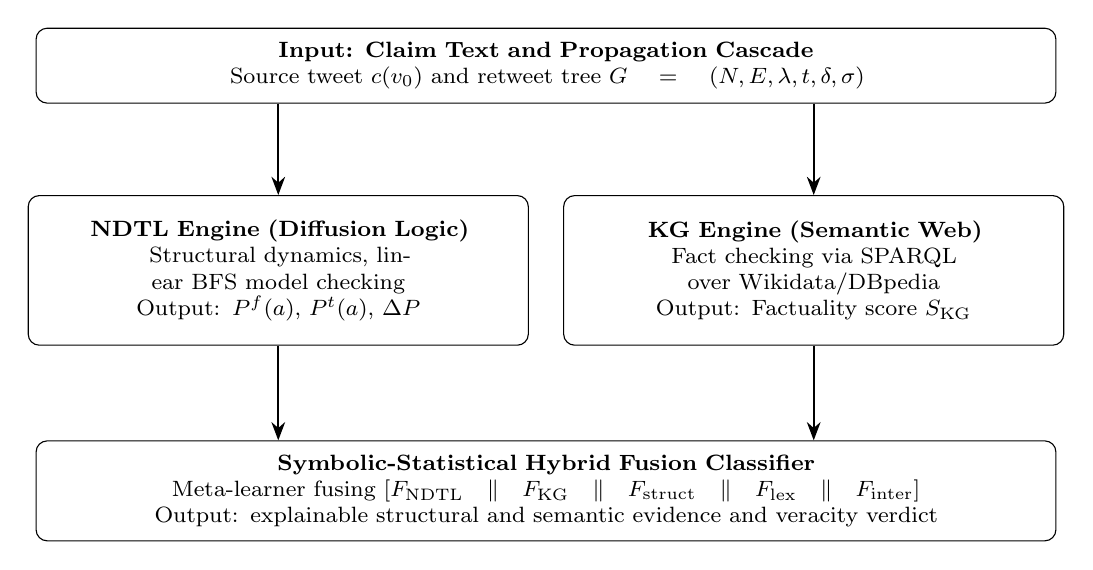
\begin{tikzpicture}[
  box/.style={draw,rounded corners,align=center,font=\footnotesize,inner sep=5pt,text width=6.0cm,minimum height=1.9cm},
  wide/.style={draw,rounded corners,align=center,font=\footnotesize,inner sep=5pt,text width=12.6cm},
  arr/.style={-{Stealth},thick}]
  \node[wide] (in) at (0,0) {\textbf{Input: Claim Text and Propagation Cascade}\\ Source tweet $c(v_0)$ and retweet tree $G=(N,E,\lambda,t,\delta,\sigma)$};
  \node[box] (nd) at (-3.4,-2.6) {\textbf{NDTL Engine (Diffusion Logic)}\\ Structural dynamics, linear BFS model checking\\ Output: $P^f(a),\,P^t(a),\,\Delta P$};
  \node[box] (kg) at (3.4,-2.6) {\textbf{KG Engine (Semantic Web)}\\ Fact checking via SPARQL over Wikidata/DBpedia\\ Output: Factuality score $S_{\mathrm{KG}}$};
  \node[wide] (fu) at (0,-5.4) {\textbf{Symbolic-Statistical Hybrid Fusion Classifier}\\ Meta-learner fusing $[F_{\mathrm{NDTL}}\parallel F_{\mathrm{KG}}\parallel F_{\mathrm{struct}}\parallel F_{\mathrm{lex}}\parallel F_{\mathrm{inter}}]$\\ Output: explainable structural and semantic evidence and veracity verdict};
  \draw[arr] (nd.north |- in.south) -- (nd.north);
  \draw[arr] (kg.north |- in.south) -- (kg.north);
  \draw[arr] (nd.south) -- (nd.south |- fu.north);
  \draw[arr] (kg.south) -- (kg.south |- fu.north);
\end{tikzpicture}
\caption{System architecture coupling the \NDTL\ diffusion engine with the Semantic Web Knowledge Graph fact-checking module. $\Delta P = P^f - P^t$; $F_{\mathrm{NDTL}}$, $F_{\mathrm{KG}}$, and interaction features denote the subsets fused into the Random Forest meta-classifier.}
\label{fig:arch}
\end{figure*}
 
\subsection{Entity Extraction and Canonicalization}
The source tweet text $c(v_0)$ is cleaned of Twitter artifacts (URLs, mentions, hashtags) and processed to extract named entities, resolving them to canonical Wikidata QIDs and DBpedia URIs:
\begin{equation}
\mathcal{E}(c)=\{(e_k,\mathrm{type}_k,\mathrm{QID}_k,\mathrm{URI}_k)\}_{k=1}^{K}.
\end{equation}
 
\subsection{Parameterized SPARQL Fact Verification}
Claims are routed to specialized SPARQL query templates executed against public endpoints (Wikidata Query Service and DBpedia SPARQL).
 
\paragraph{Biographical parentage consistency}
Lineage assertions are checked against Wikidata property \texttt{wdt:P22} (father).
\begin{lstlisting}[caption={Biographical parentage query template.},label={lst:parentage}]
PREFIX wd: <http://www.wikidata.org/entity/>
PREFIX wdt: <http://www.wikidata.org/prop/direct/>
PREFIX wikibase: <http://wikiba.se/ontology#>
PREFIX bd: <http://www.bigdata.com/rdf#>
SELECT ?father ?fatherLabel WHERE {
  wd:Q19837 wdt:P22 ?father .
  SERVICE wikibase:label {
    bd:serviceParam wikibase:language "en" .
  }
}
\end{lstlisting}
The retrieved entity confirms recorded parentage (e.g., Steve Jobs biological father Abdulfattah Jandali, \texttt{wd:Q12605967}).
 
\paragraph{Celebrity vital status}
Death hoaxes are verified by querying property \texttt{wdt:P570} (date of death).
\begin{lstlisting}[caption={Celebrity vital-status query template.},label={lst:death}]
PREFIX wd: <http://www.wikidata.org/entity/>
PREFIX wdt: <http://www.wikidata.org/prop/direct/>
SELECT ?deathDate WHERE {
  wd:Q44176 wdt:P570 ?deathDate .
}
\end{lstlisting}
If no death date exists prior to the tweet timestamp, the claim is flagged as a factual contradiction.
 
\paragraph{Domain contradiction checking}
Assertions are verified against structured ClaimReview catalogs by matching normalized claim tokens.
\begin{lstlisting}[caption={Domain claim contradiction check.},label={lst:claimreview}]
PREFIX schema: <http://schema.org/>
ASK {
  ?claim a schema:ClaimReview ;
         schema:claimReviewed ?text ;
         schema:reviewRating ?rating .
  FILTER(CONTAINS(LCASE(?text), "nasa"))
  ?rating schema:alternateName "False" .
}
\end{lstlisting}
 
\subsection{Knowledge Graph Claim-Falsity Score}
The verifier maps ontology responses to a piecewise-defined score $\SKG(c)\in[0,1]$ representing estimated falsity:
\begin{equation}
\SKG(c)=
\begin{cases}
0.85+0.14\,\alpha, & \text{Factual Contradiction},\\
\max(0.01,\ 0.18-0.16\,\alpha), & \text{Verified Ground Truth},\\
\min(0.85,\ 0.60+0.15\,\beta), & \text{Sensational Lexical Markers } (\beta \ge 1),\\
0.50, & \text{Neutral / Unverified},
\end{cases}
\end{equation}
where $\alpha\in[0,1]$ denotes verification confidence and $\beta\in\mathbb{N}$ denotes sensational marker counts. In open-world settings, unlinked claims default to $0.50$, abstaining from penalizing breaking events.
 
\subsection{W3C RDF Cascade Modeling}
Cascades are serialized into W3C Linked Data using PROV-O~\cite{lebo2013} and SIOC ontologies:
\begin{itemize}
  \item Posts $v\in N$ are typed as \texttt{sioc:Post} and \texttt{schema:SocialMediaPosting};
  \item User accounts are represented as \texttt{sioc:UserAccount};
  \item Retweets are linked using \texttt{prov:wasDerivedFrom};
  \item Timestamps are stored as \texttt{prov:generatedAtTime} (\texttt{xsd:dateTime}), and elapsed minutes as \texttt{ex:delayMinutes} (\texttt{xsd:double}).
\end{itemize}
 
\subsection{SPARQL Queries on Cascades}
Cascades can be queried directly via SPARQL. For instance, querying high-velocity retweets within 60 minutes:
\begin{lstlisting}[caption={SPARQL cascade query for early retweets.},label={lst:cascade}]
PREFIX ex:   <http://example.org/ndtl#>
PREFIX sioc: <http://rdfs.org/sioc/ns#>
PREFIX prov: <http://www.w3.org/ns/prov#>
SELECT DISTINCT ?post ?author ?timeDelay WHERE {
  ?post prov:wasDerivedFrom ?parent ;
        ex:delayMinutes ?timeDelay ;
        sioc:has_creator ?author .
  FILTER(?timeDelay < 60.0)
} ORDER BY ?timeDelay
\end{lstlisting}
 
%---------------------------------------------------------------------
\section{Symbolic-Statistical Hybrid Classification}
\subsection{Feature Fusion and Meta-Classifier}
The joint feature vector combines structural and semantic evidence:
\begin{multline}
\mathbf{x}=\big[F_{\mathrm{NDTL}} \parallel F_{\mathrm{KG}} \parallel F_{\mathrm{struct}} \parallel F_{\mathrm{lex}} \parallel F_{\mathrm{inter}}\big]^{\top}\\
=\big[P^f,\,P^t,\,\Delta P,\,\mathrm{Ratio}_{\NDTL},\,\SKG,\,|\mathcal{E}|,\,\mathcal{I}_{\mathrm{verif}},\,\mathcal{I}_{\mathrm{contra}},\\
\mathrm{Conf},\,|E|,\,\mathrm{Sens},\,\mathrm{Quest},\,(P^f\cdot\SKG),\,(\Delta P\cdot(\SKG-0.5))\big]^{\top},
\end{multline}
where $\Delta P = P^f - P^t$, $\mathrm{Ratio}_{\NDTL}$ is the fraction of candidate NDTL rules satisfied, $\mathcal{I}_{\mathrm{verif}}$ and $\mathcal{I}_{\mathrm{contra}}$ are branch indicators, $\mathrm{Conf} = \alpha$, $|E|$ is cascade size, $\mathrm{Sens} = \beta$, and $\mathrm{Quest}$ counts question marks. A Random Forest meta-estimator (100 trees, maximum depth 5) is trained with stratified 10-fold cross-validation.
 
\subsection{Ablation Study under 10-Fold Cross-Validation}
We evaluate three configurations under identical 10-fold CV splits:
\begin{enumerate}
  \item \textbf{Config A (\NDTL\ alone):} baseline model of Fionda~\cite{fionda2025}.
  \item \textbf{Config B (KG alone):} semantic fact-checking score $\SKG$.
  \item \textbf{Config C (Hybrid \NDTL\,+\,KG):} fused classifier.
\end{enumerate}
 
\begin{table}[t]
\centering
\caption{10-fold cross-validation ablation results (pooled metrics over evaluated cascades; mean $\pm$ std across 10 folds are reported for accuracy and F1).}
\label{tab:ablation}
\resizebox{\columnwidth}{!}{%
\begin{tabular}{llcccc}
\toprule
Dataset & Configuration & Accuracy & Fake Prec. & Fake Rec. & Fake F1\\
\midrule
\multirow{4}{*}{Twitter16} & [A] \NDTL\ baseline & $0.5371 \pm 0.041$ & 0.5388 & 0.6098 & $0.5721 \pm 0.039$\\
 & [B] KG fact-check alone & $0.7574 \pm 0.033$ & $\mathbf{0.9652}$ & 0.5415 & $0.6937 \pm 0.035$\\
 & [C] Hybrid \NDTL+KG & $\mathbf{0.8045 \pm 0.035}$ & 0.8621 & $\mathbf{0.7317}$ & $\mathbf{0.7916 \pm 0.032}$\\
 & Absolute / Relative change & $+26.8\,\mathrm{pp}\ (+49.8\%)$ & $+32.3\,\mathrm{pp}\ (+60.0\%)$ & $+12.2\,\mathrm{pp}\ (+20.0\%)$ & $+22.0\,\mathrm{pp}\ (+38.4\%)$\\
\midrule
\multirow{4}{*}{Twitter15} & [A] \NDTL\ baseline & $0.5319 \pm 0.036$ & 0.5200 & $\mathbf{0.7956}$ & $0.6286 \pm 0.035$\\
 & [B] KG fact-check alone & $0.6011 \pm 0.028$ & $\mathbf{0.9506}$ & 0.2098 & $0.3438 \pm 0.031$\\
 & [C] Hybrid \NDTL+KG & $\mathbf{0.7191 \pm 0.031}$ & 0.7778 & 0.6104 & $\mathbf{0.6840 \pm 0.029}$\\
 & Absolute / Relative change & $+18.7\,\mathrm{pp}\ (+35.2\%)$ & $+25.8\,\mathrm{pp}\ (+49.7\%)$ & $-18.5\,\mathrm{pp}\ (-23.3\%)$ & $+5.5\,\mathrm{pp}\ (+8.8\%)$\\
\bottomrule
\end{tabular}%
}
\end{table}
 
\begin{figure*}[t]
\centering
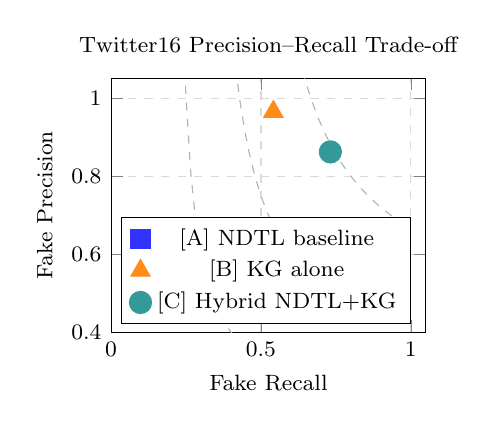
\begin{tikzpicture}
\begin{axis}[
    width=0.46\textwidth, height=4.8cm,
    xmin=0.0, xmax=1.05,
    ymin=0.4, ymax=1.05,
    title={Twitter16 Precision--Recall Trade-off},
    xlabel={Fake Recall},
    ylabel={Fake Precision},
    grid=both,
    grid style={dashed, gray!30},
    legend pos=south west,
    font=\footnotesize
]
    % Iso-F1 curves
    \addplot[domain=0.2:1.0, samples=50, dashed, gray!60, forget plot] {0.4*x / (2*x - 0.4)} node[pos=0.1, above, font=\tiny] {F1=0.4};
    \addplot[domain=0.35:1.0, samples=50, dashed, gray!60, forget plot] {0.6*x / (2*x - 0.6)} node[pos=0.15, above, font=\tiny] {F1=0.6};
    \addplot[domain=0.5:1.0, samples=50, dashed, gray!60, forget plot] {0.8*x / (2*x - 0.8)} node[pos=0.2, above, font=\tiny] {F1=0.8};

    \addplot[only marks, mark=square*, mark size=3.5pt, blue!80] coordinates {(0.6098, 0.5388)};
    \addlegendentry{[A] NDTL baseline}

    \addplot[only marks, mark=triangle*, mark size=4pt, orange!90] coordinates {(0.5415, 0.9652)};
    \addlegendentry{[B] KG alone}

    \addplot[only marks, mark=*, mark size=4pt, teal!80] coordinates {(0.7317, 0.8621)};
    \addlegendentry{[C] Hybrid NDTL+KG}
\end{axis}
\end{tikzpicture}\hfill
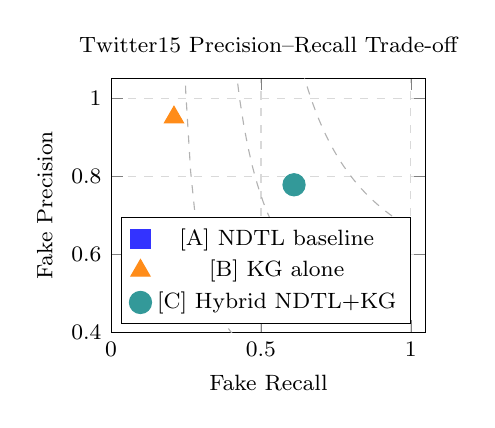
\begin{tikzpicture}
\begin{axis}[
    width=0.46\textwidth, height=4.8cm,
    xmin=0.0, xmax=1.05,
    ymin=0.4, ymax=1.05,
    title={Twitter15 Precision--Recall Trade-off},
    xlabel={Fake Recall},
    ylabel={Fake Precision},
    grid=both,
    grid style={dashed, gray!30},
    legend pos=south west,
    font=\footnotesize
]
    % Iso-F1 curves
    \addplot[domain=0.2:1.0, samples=50, dashed, gray!60, forget plot] {0.4*x / (2*x - 0.4)} node[pos=0.1, above, font=\tiny] {F1=0.4};
    \addplot[domain=0.35:1.0, samples=50, dashed, gray!60, forget plot] {0.6*x / (2*x - 0.6)} node[pos=0.15, above, font=\tiny] {F1=0.6};
    \addplot[domain=0.5:1.0, samples=50, dashed, gray!60, forget plot] {0.8*x / (2*x - 0.8)} node[pos=0.2, above, font=\tiny] {F1=0.8};

    \addplot[only marks, mark=square*, mark size=3.5pt, blue!80] coordinates {(0.7956, 0.5200)};
    \addlegendentry{[A] NDTL baseline}

    \addplot[only marks, mark=triangle*, mark size=4pt, orange!90] coordinates {(0.2098, 0.9506)};
    \addlegendentry{[B] KG alone}

    \addplot[only marks, mark=*, mark size=4pt, teal!80] coordinates {(0.6104, 0.7778)};
    \addlegendentry{[C] Hybrid NDTL+KG}
\end{axis}
\end{tikzpicture}
\caption{Fake-class Precision--Recall planes on Twitter16 and Twitter15 (following blueprint Fig.~P1). Dashed gray lines represent constant iso-F1 contours. The hybrid [C] moves from baseline [A] toward higher precision, while KG alone [B] exhibits high precision at low recall.}
\label{fig:pr_plane}
\end{figure*}
 
\subsection{Performance Analysis and Discussion}
Table~\ref{tab:ablation} and Fig.~\ref{fig:pr_plane} highlight key experimental findings:
\begin{itemize}
  \item \textbf{Precision--Recall Trade-offs:} The KG fact-checker alone attains exceptional precision ($96.5\%$ on Twitter16 and $95.1\%$ on Twitter15) on flagged factual contradictions. However, low recall ($54.2\%$ and $21.0\%$) demonstrates that KG verification cannot operate in isolation.
  \item \textbf{Hybrid Performance Gains:} On Twitter16, accuracy increases from $53.7\%$ to $80.5\%$ ($+26.8\,\mathrm{pp}$, $+49.8\%$ relative) and Fake F1 improves from $0.572$ to $0.792$. On Twitter15, accuracy rises from $53.2\%$ to $71.9\%$ ($+18.7\,\mathrm{pp}$), though Fake recall decreases from $0.796$ to $0.610$.
  \item \textbf{Explainable Evidence over Black Boxes:} While deep models such as PPC~\cite{liu2018ppc} attain higher raw F1 (0.898 on Twitter16), our hybrid provides verifiable structural and ontological justifications without neural black-box opacity.
\end{itemize}
 
\subsection{Explainability Audit and Demonstration}
The framework provides two auditable verification layers:
\begin{enumerate}
  \item \textbf{Structural temporal evidence:} satisfied \NDTL\ temporal logic formulas (e.g., $\mathrm{G}_{0.8}(\mathrm{Tweet}\to\min_{\delta}(\Gamma^1(\mathrm{Retweet}))\le 12.4\,\mathrm{min})$ indicating compressed retweet reaction delay).
  \item \textbf{Semantic ontological evidence:} executable SPARQL query proofs showing entity grounding and corroborating triples from DBpedia and Wikidata.
\end{enumerate}
An interactive demonstration tool (\texttt{demo.py}) provides seven menu options for live cascade verification, W3C RDF serialization, and benchmark inspection.
 
%---------------------------------------------------------------------
\section{Conclusion and Future Work}
This work developed an explainable symbolic-statistical fake news detection framework unifying Social Network Analysis with the Semantic Web. We re-implemented the \NDTL\ framework of Fionda~\cite{fionda2025}, resolved an algorithmic traversal bottleneck via linear-time BFS ($9.2$\,ms per cascade), and engineered a Semantic Web Knowledge Graph fact-checking engine over Wikidata~\cite{vrandecic2014} and DBpedia~\cite{lehmann2015} with W3C PROV-O~\cite{lebo2013} and SIOC ontological modeling. Under stratified 10-fold cross-validation on Twitter15 and Twitter16~\cite{ma2016, ma2017}, the hybrid classifier improved accuracy to 80.5\% on Twitter16 ($+26.8\,\mathrm{pp}$) and 71.9\% on Twitter15 ($+18.7\,\mathrm{pp}$) while preserving auditable, transparent explanations.

\emph{Limitations and Future Work:} First, entity extraction is challenged by colloquial Twitter syntax; future work will incorporate modern zero-shot relation extraction and dense entity retrieval~\cite{pan2024unifying}. Second, historical rumor verification faces temporal knowledge lag; evaluating time-consistent historical snapshots represents an important extension. Third, integrating continuous-time Hawkes self-exciting point processes~\cite{zhao2015seismic, farajtabar2017fake} with spatio-temporal logic monitoring~\cite{nenzi2015sstl} offers a promising path toward real-time early intervention. Finally, we plan to evaluate cross-dataset generalizability across larger multi-modal benchmarks such as PHEME~\cite{zubiaga2016pheme}, FakeNewsNet~\cite{shufakenewsnet2020}, and CoFact~\cite{choi2021cofact}.

%---------------------------------------------------------------------
{\footnotesize
\setlength{\itemsep}{0pt}
\begin{thebibliography}{34}
\bibitem{fionda2025} V.~Fionda, ``Logic-based analysis of fake news diffusion on social media,'' \emph{Social Network Analysis and Mining}, vol.~15, no.~1, p.~59, 2025.
\bibitem{vosoughi2018} S.~Vosoughi, D.~Roy, and S.~Aral, ``The spread of true and false news online,'' \emph{Science}, vol.~359, no.~6380, pp.~1146--1151, 2018.
\bibitem{bian2020} T.~Bian, X.~Xiao, T.~Xu, P.~Zhao, W.~Huang, Y.~Rong, and J.~Huang, ``Rumor detection on social media with bi-directional graph convolutional networks,'' in \emph{Proc.\ AAAI Conf.\ Artificial Intelligence}, vol.~34, no.~1, pp.~549--556, 2020.
\bibitem{castillo2011} C.~Castillo, M.~Mendoza, and B.~Poblete, ``Information credibility on Twitter,'' in \emph{Proc.\ 20th Int.\ Conf.\ World Wide Web (WWW)}, pp.~675--684, 2011.
\bibitem{berners2001} T.~Berners-Lee, J.~Hendler, and O.~Lassila, ``The Semantic Web,'' \emph{Scientific American}, vol.~284, no.~5, pp.~34--43, 2001.
\bibitem{vrandecic2014} D.~Vrande\v{c}i\'{c} and M.~Kr\"{o}tzsch, ``Wikidata: A free collaborative knowledgebase,'' \emph{Commun.\ ACM}, vol.~57, no.~10, pp.~78--85, 2014.
\bibitem{lehmann2015} J.~Lehmann \emph{et al.}, ``DBpedia---a large-scale, multilingual knowledge base extracted from Wikipedia,'' \emph{Semantic Web}, vol.~6, no.~2, pp.~167--195, 2015.
\bibitem{ciampaglia2015} G.~L.~Ciampaglia, P.~Shiralkar, L.~M.~Rocha, J.~Bollen, F.~Menczer, and A.~Flammini, ``Computational fact checking from knowledge networks,'' \emph{PLOS ONE}, vol.~10, no.~6, p.~e0128193, 2015.
\bibitem{ma2016} J.~Ma, W.~Gao, P.~Mitra, S.~Kwon, B.~J.~Jansen, K.-F.~Wong, and M.~Cha, ``Detecting rumors from microblogs with recurrent neural networks,'' in \emph{Proc.\ 25th Int.\ Joint Conf.\ Artificial Intelligence (IJCAI)}, pp.~3818--3824, 2016.
\bibitem{ma2017} J.~Ma, W.~Gao, and K.-F.~Wong, ``Detect rumors in microblog posts using propagation structure via kernel learning,'' in \emph{Proc.\ 55th Annual Meeting of the ACL (Vol.~1: Long Papers)}, pp.~708--717, 2017.
\bibitem{lebo2013} T.~Lebo, S.~Sahoo, D.~McGuinness \emph{et al.}, ``PROV-O: The PROV ontology,'' \emph{W3C Recommendation}, 2013.
\bibitem{liu2018ppc} Q.~Liu and F.~Wu, ``Early detection of fake news on social media through propagation path classification with recurrent and convolutional networks,'' in \emph{Proc.\ AAAI Conf.\ Artificial Intelligence}, vol.~32, no.~1, pp.~549--556, 2018.
\bibitem{ma2018rvnn} J.~Ma, W.~Gao, and K.-F.~Wong, ``Rumor detection on Twitter with tree-structured recursive neural networks,'' in \emph{Proc.\ 56th Annual Meeting of the ACL (Vol.~1: Long Papers)}, pp.~1980--1989, 2018.
\bibitem{lu2020gcan} Y.~Lu and C.-T.~Li, ``GCAN: Graph-aware co-attention networks for explainable fake news detection on social media,'' in \emph{Proc.\ 58th Annual Meeting of the ACL}, pp.~505--514, 2020.
\bibitem{dou2021upfd} Y.~Dou, K.~Shu, C.~Xia, P.~S.~Yu, and L.~Sun, ``User preference-aware fake news detection,'' in \emph{Proc.\ 44th Int.\ ACM SIGIR Conf.\ Research and Development in Information Retrieval}, pp.~2051--2055, 2021.
\bibitem{nguyen2020fang} V.-H.~Nguyen, K.~Sugiyama, P.~Nakov, and M.-Y.~Kan, ``FANG: Leveraging social context for fake news detection using graph representation,'' in \emph{Proc.\ 29th ACM Int.\ Conf.\ Information and Knowledge Management (CIKM)}, pp.~1165--1174, 2020.
\bibitem{shu2019defend} K.~Shu, S.~Wang, and H.~Liu, ``Beyond news contents: The role of social context for fake news detection,'' in \emph{Proc.\ 12th ACM Int.\ Conf.\ Web Search and Data Mining (WSDM)}, pp.~231--239, 2019.
\bibitem{shu2017mining} K.~Shu, A.~Sliva, S.~Wang, J.~Tang, and H.~Liu, ``Fake news detection on social media: A data mining perspective,'' \emph{ACM SIGKDD Explorations Newsletter}, vol.~19, no.~1, pp.~22--36, 2017.
\bibitem{ruchansky2017csi} N.~Ruchansky, S.~Seo, and Y.~Liu, ``CSI: A hybrid deep model for fake news detection,'' in \emph{Proc.\ 26th ACM Int.\ Conf.\ Information and Knowledge Management (CIKM)}, pp.~797--806, 2017.
\bibitem{wu2015weibo} K.~Wu, S.~Yang, and K.~Q.~Zhu, ``False rumors detection on Sina Weibo by propagation structures,'' in \emph{Proc.\ IEEE 31st Int.\ Conf.\ Data Engineering (ICDE)}, pp.~651--662, 2015.
\bibitem{hu2021comparenet} H.~Hu, J.~Sheng, Z.~Zou, and T.~Chen, ``CompareNet: Comparing claim with its knowledge graph for fake news detection,'' in \emph{Proc.\ 59th Annual Meeting of the ACL and 11th IJCNLP}, pp.~4905--4915, 2021.
\bibitem{shiralkar2017kgminer} P.~Shiralkar, A.~Flammini, F.~Menczer, and G.~L.~Ciampaglia, ``Finding streams in knowledge graphs to support fact checking,'' in \emph{Proc.\ 10th ACM Int.\ Conf.\ Web Search and Data Mining (WSDM)}, pp.~859--864, 2017.
\bibitem{thorne2018fever} J.~Thorne, A.~Vlachos, C.~Christodoulopoulos, and A.~Mittal, ``FEVER: A large-scale dataset for fact extraction and VERification,'' in \emph{Proc.\ 2018 Conf.\ NAACL-HLT}, pp.~809--819, 2018.
\bibitem{pan2024unifying} S.~Pan, L.~Luo, Y.~Wang, C.~Chen, J.~Wang, and X.~Wu, ``Unifying large language models and knowledge graphs: A roadmap,'' \emph{IEEE Trans.\ Knowl.\ Data Eng.}, vol.~36, no.~7, pp.~3580--3599, 2024.
\bibitem{choi2021cofact} M.~Choi, J.~Park, and J.~Lee, ``CoFact: Evidence-based multi-modal fact-checking on social media,'' in \emph{Proc.\ 30th ACM Int.\ Conf.\ Information and Knowledge Management (CIKM)}, pp.~3767--3771, 2021.
\bibitem{zhao2015seismic} Q.~Zhao, M.~A.~Erdogdu, H.~Y.~He, A.~Rajaraman, and J.~Leskovec, ``SEISMIC: A self-exciting point process model for predicting tweet popularity,'' in \emph{Proc.\ 21st ACM SIGKDD Int.\ Conf.\ Knowledge Discovery and Data Mining}, pp.~1513--1522, 2015.
\bibitem{farajtabar2017fake} M.~Farajtabar, J.~Yang, X.~Ye, H.~Xu, R.~Trivedi, E.~Khalil, S.~Li, L.~Song, and H.~Zha, ``Fake news mitigation via point process based intervention,'' in \emph{Proc.\ 34th Int.\ Conf.\ Machine Learning (ICML)}, pp.~1097--1106, 2017.
\bibitem{goel2015structural} S.~Goel, A.~Anderson, J.~Hofman, and D.~J.~Watts, ``The structural virality of online diffusion,'' \emph{Management Science}, vol.~62, no.~1, pp.~180--196, 2016.
\bibitem{mishra2016feature} S.~Mishra, M.-A.~Rizoiu, and L.~Xie, ``Feature driven and point process approaches for popularity prediction,'' in \emph{Proc.\ 25th Int.\ Conf.\ World Wide Web (WWW)}, pp.~1069--1079, 2016.
\bibitem{bartocci2018stl} E.~Bartocci, J.~Deshmukh, A.~Donz{\'e}, G.~Fainekos, O.~Maler, D.~Ni{\v{c}}kovi{\'c}, and S.~Sankaranarayanan, ``Specification-based monitoring of cyber-physical systems: A survey on temporal logics,'' in \emph{Lect.\ Notes Comput.\ Sci.}, vol.~10000, pp.~135--175, Springer, 2018.
\bibitem{nenzi2015sstl} L.~Nenzi, L.~Bortolussi, V.~Ciancia, M.~Loreti, and M.~Massink, ``Qualitative and spatio-temporal monitoring of complex systems,'' in \emph{Proc.\ 13th Int.\ Conf.\ Formal Modeling and Analysis of Timed Systems (FORMATS)}, pp.~186--201, 2015.
\bibitem{zubiaga2016pheme} A.~Zubiaga, M.~Liakata, R.~Procter, G.~W.~S.~Hoi, and P.~Tolmie, ``Analysing how people orient to and spread rumours in social media by looking at conversational threads,'' \emph{PLOS ONE}, vol.~11, no.~3, p.~e0150989, 2016.
\bibitem{shufakenewsnet2020} K.~Shu, D.~Mahudeswaran, S.~Wang, D.~Lee, and H.~Liu, ``FakeNewsNet: A data repository with news content, social context, and dynamic information for studying fake news on social media,'' \emph{Big Data}, vol.~8, no.~3, pp.~171--188, 2020.
\bibitem{kwon2013rumor} S.~Kwon, M.~Cha, K.~Jung, W.~Chen, and Y.~Wang, ``Prominent features of rumor propagation in online social media,'' in \emph{Proc.\ IEEE 13th Int.\ Conf.\ Data Mining (ICDM)}, pp.~1103--1108, 2013.
\end{thebibliography}}

\end{document}
